\subsection{\emph{Image Viewer Node}}
\label{subsec:imageviewernode}

\emph{Image viewer node} merupakan \emph{behavior node} yang digunakan untuk melihat tampilan dari data citra yang dikirimkan pada suatu \emph{topic}.
\emph{Image viewer node} yang digunakan ini merupakan program \lstinline{rqt_image_view} yang berasal dari \emph{package} \lstinline{rqt_image_view}.
\emph{Node} tersebut akan menerima data citra pada suatu \emph{topic} yang memiliki \emph{interface} \lstinline{sensor_msgs/msg/Image},
  dan kemudian menampilkannya dalam bentuk GUI.

\begin{figure}[ht]
  \centering
  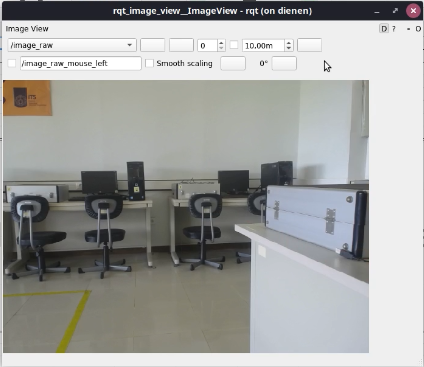
\includegraphics[scale=0.55]{gambar/tampilan-image-viewer.png}
  \caption{Tampilan GUI dari \emph{image viewer node}.}
  \label{fig:tampilanimageviewer}
\end{figure}

Seperti yang terlihat pada gambar \ref{fig:tampilanimageviewer},
  \emph{Node} tersebut memiliki tampilan GUI yang dapat digunakan untuk memilih \emph{topic} dari data citra yang akan ditampilkan.
Jika \emph{image viewer node} mendapatkan data yang berasal dari \emph{topic} tersebut,
  \emph{node} tersebut akan memproses data yang diterima serta menampilkannya dalam bentuk GUI.
Selain itu \emph{node} ini juga bisa digunakan untuk menyimpan data citra yang diterima tersebut dalam bentuk file gambar.
